% fig4_benchmark_overhead.tex — Figure 5 (column width)
% BTV governance overhead vs. typical AI inference latency, log scale.
% Regenerated 2026-09-15 (COMSI-2026-04-0112 R1) with the committed
% G5-corrected collection: data/sweep_raw_20260915T024430Z_g5fix.csv
% (medians at 4 KiB, one thread). The LLM inference bar is an
% order-of-magnitude reference, not a measurement.
\documentclass[border=2pt]{standalone}
\usepackage{pgfplots}
\pgfplotsset{compat=1.18}
\begin{document}
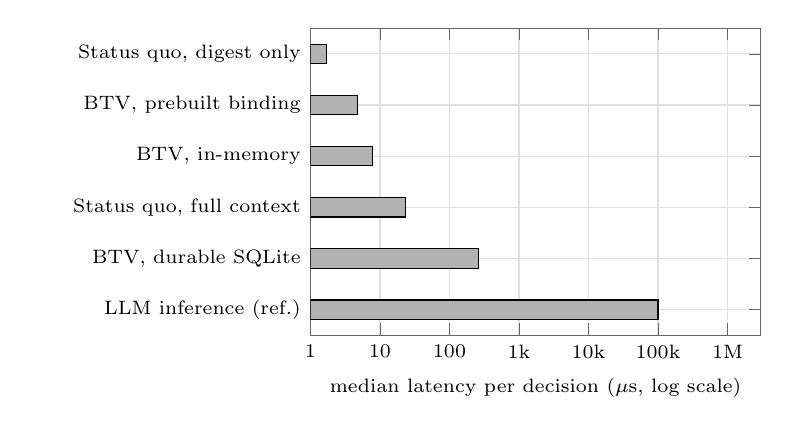
\begin{tikzpicture}[font=\footnotesize]
\begin{axis}[
  xmode=log,
  log basis x=10,
  xmin=1, xmax=3e6,
  width=7.3cm,
  height=6.4cm,
  bar width=7pt,
  y=6.5mm,
  ytick=data,
  symbolic y coords={
    {LLM inference (ref.)},
    {BTV, durable SQLite},
    {Status quo, full context},
    {BTV, in-memory},
    {BTV, prebuilt binding},
    {Status quo, digest only}},
  yticklabel style={font=\scriptsize, text width=3.35cm, align=right},
  xtick={1,10,100,1000,10000,100000,1000000},
  xticklabels={1,10,100,{1k},{10k},{100k},{1M}},
  xticklabel style={font=\scriptsize},
  xlabel={median latency per decision ($\mu$s, log scale)},
  xlabel style={font=\scriptsize},
  log ticks with fixed point,
  grid=both,
  grid style={black!12},
  axis line style={black!60},
  tick style={black!60},
  every axis plot/.append style={draw=black, fill=black!30},
]
\addplot+[xbar, mark=none, draw=black, fill=black!30]
  coordinates {(1.68,{Status quo, digest only})
               (4.69,{BTV, prebuilt binding})
               (7.82,{BTV, in-memory})
               (23.61,{Status quo, full context})
               (261.44,{BTV, durable SQLite})
               (100000,{LLM inference (ref.)})};
\end{axis}
\end{tikzpicture}
\end{document}
